%%%%%%%%%%%%%%%%%%%%%%%%%%
%%% author : Yamada. T %%%
%%% made for TH series %%%
%%%%%%%%%%%%%%%%%%%%%%%%%%

\documentclass[b5paper,10pt,fleqn] {ltjsarticle}

\usepackage[margin=10truemm]{geometry}

\usepackage{pict2e, graphicx}
\usepackage{tikz}
\usetikzlibrary{intersections,calc,arrows.meta}

\usepackage{amsmath, amssymb, amsthm}
\usepackage{ascmac}
\usepackage{comment}
\usepackage{empheq}
\usepackage[shortlabels,inline]{enumitem}
\usepackage{fancybox}
\usepackage{fancyhdr}
\usepackage{here}
\usepackage{lastpage}
\usepackage{listings, jvlisting}
\usepackage{fixdif}

\usepackage{stmaryrd}
\usepackage[listings]{tcolorbox}
%\usepackage{ascolorbox}
\usepackage{titlesec}
\usepackage{ulem}
\usepackage{url}
\usepackage{verbatim}
\usepackage{wrapfig}
\usepackage{xcolor}
\usepackage{luatexja-ruby}
\usepackage{varwidth}
\usepackage[version=3]{mhchem}
\usepackage{wrapfig}


\usepackage{physics2}
	\usephysicsmodule{ab}
	\usephysicsmodule{ab.braket}
	\usephysicsmodule{ab.legacy}
	%\usephysicsmodule{braket}
	\usephysicsmodule{diagmat}
	\usephysicsmodule{xmat}
	\usephysicsmodule{nabla.legacy}
	\usephysicsmodule{qtext.legacy}

\usepackage[ISO]{diffcoeff}
\difdef { f, s } { D }
{ op-symbol = \mathrm{D} }


\newcommand{\mctext}[1]{\mbox{\textcircled{\scriptsize{#1}}}}
\newcommand{\ctext}[1]{\textcircled{\scriptsize{#1}}}
\newcommand{\ds}{\displaystyle}
\newcommand{\comb}[2]{{}_{#1}\mathrm{C}_{#2}}
\newcommand{\hs}{\hspace}
\newcommand{\vs}{\vspace}
\newcommand{\emphvs}{\vspace{1em}\notag\\}
\newcommand{\ora}{\overrightarrow}
\newcommand{\oramr}[1]{\overrightarrow{\mathrm{#1}}}
\newcommand{\tri}{\triangle}
\newcommand{\mr}{\mathrm}
\newcommand{\mb}{\mathbb}
\newcommand{\mrvec}[1]{\overrightarrow{\mathrm{#1}}}
\newcommand{\itvec}{\overrightarrow}
\newcommand{\bs}{\boldsymbol}
\newcommand{\ra}{\rightarrow}
\newcommand{\Ra}{\Rightarrow}
\newcommand{\lra}{\longrightarrow}
\newcommand{\Lra}{\Longrightarrow}
\newcommand{\la}{\leftarrow}
\newcommand{\La}{\Leftarrow}
\newcommand{\lla}{\longleftarrow}
\newcommand{\Lla}{\Longleftarrow}
\newcommand{\lr}{\leftrightarrow}
\newcommand{\llr}{\longleftrightarrow}
\newcommand{\Llr}{\Longleftrightarrow}
\renewcommand{\deg}{{}^\circ}
\newcommand{\phbox}{\fbox{\phantom{1\hspace{2em}}}}
\newcommand{\boxnum}[1]{\fbox{\phantom{\hspace{1em}}({#1})\phantom{\hspace{1em}}}}
\newcommand{\boxkana}[1]{\fbox{\phantom{\hspace{1em}}{#1}\phantom{\hspace{1em}}}}
\newcommand{\boxkm}[2]{\fbox{\, {#1}\phantom{\hspace{0.2em}} \,  ${#2}$}}
\newcommand{\hzw}{\hspace{1\zw}}

\renewcommand{\baselinestretch}{1.25}
\parindent=1\zw


\begin{document}
\noindent\fbox{成仏シテクレ←入88}

\begin{wrapfigure}{r}{5cm}
  \centering
  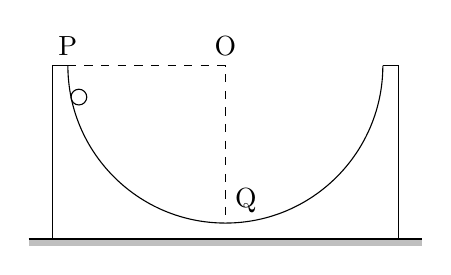
\begin{tikzpicture}
    \draw (-2, 0) arc[radius=2, start angle=180, end angle=360];
    \draw (-2,0)--(-2.2,0)--(-2.2,-2.2)--(2.2,-2.2)--(2.2,0)--(2,0);
    \draw [dashed] (-2,0)--(0,0)--(0,-2);
    \filldraw [fill=lightgray,draw=white] (-2.5,-2.2)--(2.5,-2.2)--(2.5,-2.3)--(-2.5,-2.3)--cycle;
    \draw [semithick] (-2.5,-2.2)--(2.5,-2.2);
    \draw [above] (0,0) node {O};
    \draw [above] (-2,0) node {P};
    \draw [above right] (0,-2) node {Q};
    \draw (-1.86,-0.4) circle[radius=0.1];
  \end{tikzpicture}
\end{wrapfigure}

なめらかで水平な床の上に,内面に半径$r$の半円形のレールを取り付けた台が置かれている.
レール上に置かれた質量$m$の小球は,摩擦なしにレールの上を動くことができる.
台の質量は$5m$であり,台,および小球の運動は,紙面内のみで行われる.
重力加速度の大きさを$g$とし,以下の各問いに答えよ.
\begin{enumerate}[label={\textbf{問\arabic*}}]
  \item {\hzw}台を固定し,動かないようにしておく.点Pに小球を静かに置くと,小球はレール上を下り始め,やがてレールの最下点Qを通過した.
  \begin{enumerate}[(1)]
    \item {\hzw}Qを通過する瞬間の床から見た小球の速さはいくらか.
    \item {\hzw}Qを通過する瞬間の小球がレールから受ける垂直抗力の大きさはいくらか.
  \end{enumerate}
  \item {\hzw}台の固定を解く.Pに小球を置き,台と小球を手で支えて静止させた状態から静かに手をはなすと,台,小球はいずれも動き始め,やがて小球はQを通過した.
  \begin{enumerate}[(1), resume]
    \item {\hzw}Qを通過する瞬間の床から見た小球の速さはいくらか.
    \item {\hzw}Qを通過する瞬間の小球がレールから受ける垂直抗力の大きさはいくらか.
    \item {\hzw}手をはなした瞬間から小球がQを通過するまでの間に,台は左向きに最初の位置からどれだけ動いたか.ただし,台の重心はQを通る鉛直線上にあるものとする.
  \end{enumerate}
  \item {\hzw}台を静止させ,Qに小球を置いた.この状態から台に外力を水平方向に加え,一定の加速度で台を右向きに加速させた.加速を開始してから時間$T$の後に,小球はPから飛び出し,Pより鉛直上方に$\dfrac{r}{2}$の高さにまで達した後に落下した.
  \begin{enumerate}[(1), resume]
    \item {\hzw}このような水平方向の加速で,Pから小球を飛び出させるためには加速度の大きさがいくらより大きいことが必要か.
    \item {\hzw}Pから飛び出したときの小球の鉛直方向の速さはいくらか.
    \item {\hzw}台の水平方向の加速度の大きさはいくらか.
    \item {\hzw}Pから飛び出す直前に,小球がレールから受けていた垂直抗力の大きさはいくらか.
    \item {\hzw}加速開始よりPから小球が飛び出すまでの時間$T$の間に,外力がした仕事はいくらか.答えには文字$T$を用いてよい.
  \end{enumerate}

\end{enumerate}




\end{document}